\documentclass[12pt, a4paper]{article}
\usepackage[german,ngerman]{babel}
\usepackage[babel,german=quotes]{csquotes} % deutsche Anführungszeichen
\usepackage{graphicx}
\usepackage{float}
\usepackage[T1]{fontenc}
\usepackage{bibgerm}	%Unterstützung für bibtex, mehrere Autorennamen mit "and"
%\usepackage{lmodern}
\usepackage{hyperref}
\usepackage[utf8]{inputenc}

\usepackage[left=3cm, right=3cm, top=2cm, bottom=2cm, includeheadfoot]{geometry}
%\usepackage{geometry}
%\geometry{verbose,a4paper,tmargin=10mm,bmargin=10mm,lmargin=30mm,rmargin=30mm}

%% alle serifenlosen Teile des Dokuments in Helvetica gesetzt
\usepackage{helvet}

\setcounter{section}{0}

%% Zeilenabstand
\linespread{1.00}

\bibliographystyle{unsrt}	%zitatangabe


%% Schriftformatierung der einzelnen Elemente wie Überschrift usw.
%\setkomafont{chapter}{\sffamily \Large}
%\setkomafont{section}{\sffamily \textit}
%\setkomafont{subsection}{\sffamily \textit}


\begin{document}
	
		%% Deckplatt generieren
	\begin{titlepage}
		\centering
		{\sffamily\huge Fachbereich 07 Informatik/Mathematik \par}
		
\includegraphics[width=0.5\textwidth]{images/Hochschule_Muenchen_Logo.png}\par
		\vspace{1cm}
		{\sffamily\LARGE Praktikum Datenschutz und Datensicherheit Sommersemester 2016\par}
		\vspace{1cm}
		{\sffamily\Large Prof. Dr. Rainer W. Gerling\par}
		{\sffamily\Large Heidi Schuster\par}
		\vspace{2cm}
		{\LARGE Man-in-the-Middle\par}
		\vspace{1.5cm}
		{\LARGE Fabian Uhlmann\par}
		{\LARGE IF6\par}
		\vspace{0.5cm}
		{\LARGE Diana Irmscher\par}
		{\LARGE IF7\par}
		\vspace{1cm}
		{\large \today\par}
		% Ende der Titelseite
		\vfill
	\end{titlepage}
	
	\section*{Abstract}
Im Rahmen des Studiums Bachelor Informatik absolvieren wir (Fabian Uhlmann und Diana Irmscher) die zusätzliche Ausbildung zum betrieblichen Datenschutz an der Hochschule München.
\\
Das Thema Datenschutz und IT-Sicherheit ist in den letzten Jahren immer mehr in den Vordergrund getreten. Medien berichten fast täglich über diverse Angriffe wie z. B. auf den Bundestag im Mai 2015 oder aktuell über den Krypto-Trojaner Locky.
\\	
Wir haben das Thema "'Man-in-the-Middle"' gewählt, weil es sich dabei um Angriffsszenarien handelt, die jeden vernetzten Nutzer jederzeit treffen können.
%TODO ggf. hier Aufgbau der Ausarbeitung
\\	
Das Thema ist in zwei Unterthemen aufgeteilt.
Herr Uhlmann wird darauf eingehen, wie man die Sicherheit eines Systems mit einem MITM-Angriff sehr effizient aushebeln kann.
Frau Irmscher beschäftigt sich mit dem gezielten Angriff in TLS/SSL und in gesnifften Netzwerken.
{\flushright{München, \today}}
		 

	\newpage

	\tableofcontents		%Macht das Inhaltsverzeichnis
	\newpage
	
	%% Fabian
	\section*{Aufgabenstellung}
\addcontentsline{toc}{section}{Aufgabenstellung}
Dell und Lenovo haben demonstriert, dass man mit Man-in-the-Middle
Angriffen die Sicherheit eines Systems sehr effizient aushebeln kann.
Wie funktioniert ein derartiger Angriff und was kann man tun, um sich
zu schützen.

	\subsection{Bedeutung einer Man-in-the-Middle Attacke}
Man in the Middle (MITM) ist ein Angriffsszenario, bei der ein unberechtigter Dritter versucht, in eine zwischen zwei Kommunikationspartnern geführte, sichere (verschlüsselte) oder auch unsichere (unverschlüsselte) Kommunikation einzudringen. Ziel des Angreifers ist es, die zu übertragenden, vertraulichen Informationen unbemerkt mitzulesen und/oder zu manipulieren. Um unerkannt im Hintergrund an die Daten beziehungsweise Informationen zu gelangen, täuscht der Angreifer vor, der jeweilige andere Kommunikationspartner zu sein. Ein MITM-Angriff kann auf den verschiedenen Ebenen des ISO/OSI Schichten-Modells \cite[vgl.]{osi}, z. B. auf Anwendungsebene (HTTP/HTTPs) oder Netzwerkebene (IP) stattfinden. Quelle: \cite[vgl.]{mitm-def}
\begin{figure}[H]
	\centering
	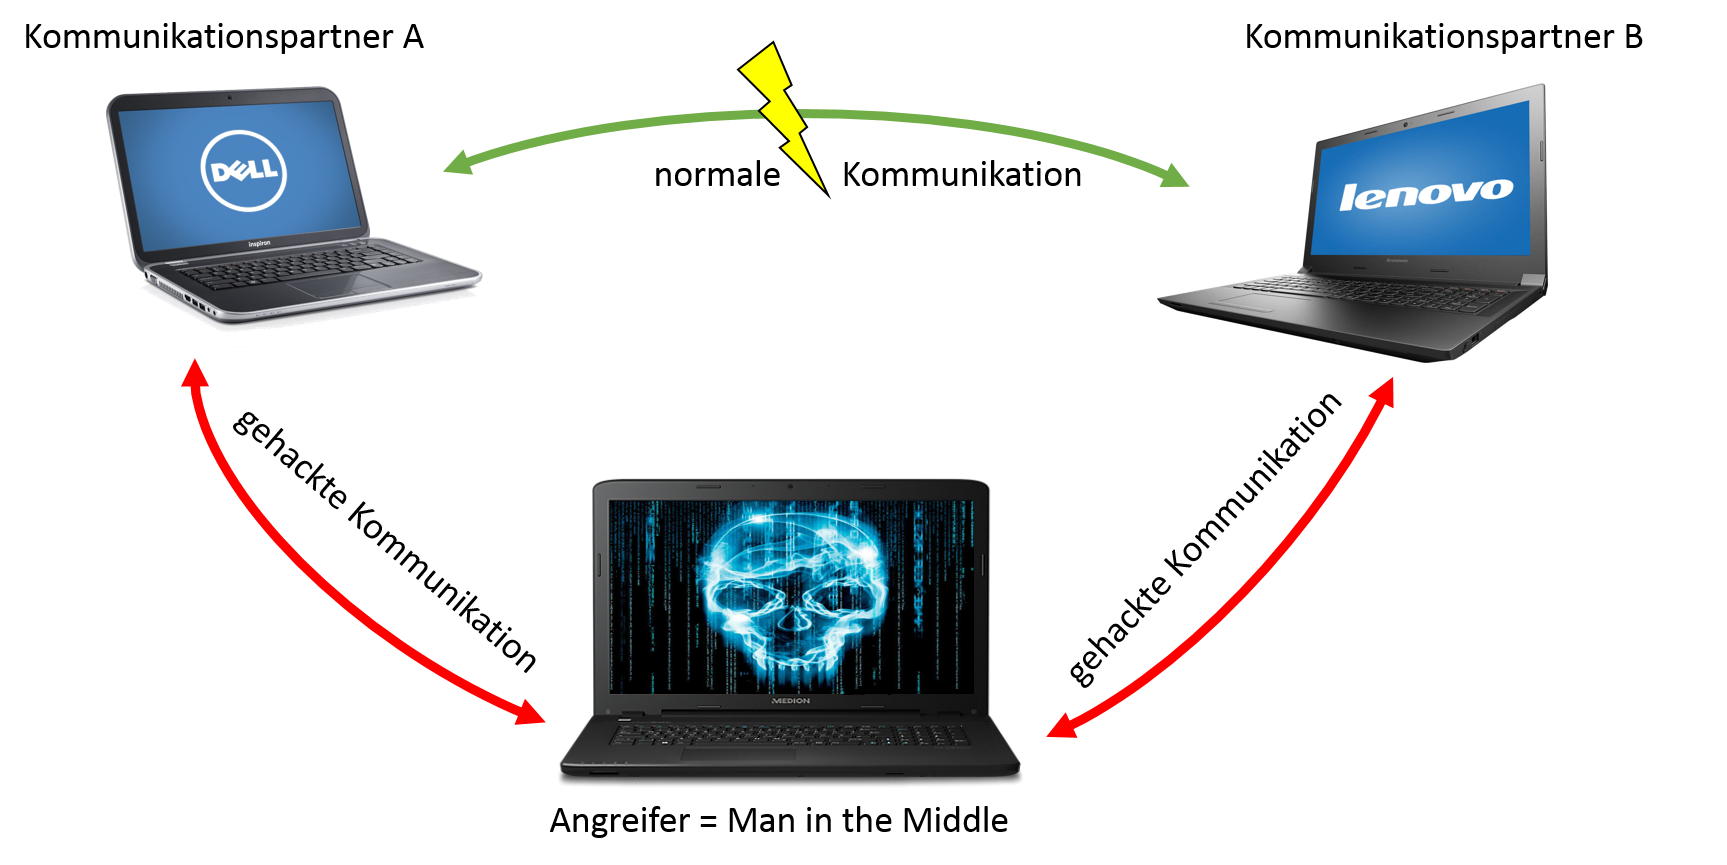
\includegraphics[width=.8\linewidth]{images/MITM.png}
	\caption{Man in the Middle Angriff \cite{mitm-bild}}
\end{figure}
	\section{Zusammenhang HTTP(s) und Zertifikate}
\label{sec:HTTPs}
Typischerweise fragt ein Nutzer eine Internetseite über das unsichere Hypertext Transfer Protocol (HTTP) an. Dabei werden alle benötigten Informationen wie z. B. Benutzername und Passwort im Klartext übermittelt. Ebenfalls wird die Rückantwort unverschlüsselt übertragen. Für einen sicheren Datenaustausch sollte ein Anwender, falls dies angeboten wird, die Internetseite per Hypertext Transfer Protocol Secure (HTTPs) aufrufen. \cite[vgl.]{RFC7230} 
\\Seriöse Online-Banking-Webseiten unterstützen beispielsweise nur noch HTTPs-Aufrufe. Dabei wird dem Aufruf durch das Kürzel HTTPs in der Adressleiste signalisiert, dass es sich hierbei um eine verschlüsselte Verbindung handelt. Bei jeder HTTPs-Kommunikation muss sich der Webserver, auf dem die Internetseite gehostet wird, authentifizieren. Die Authentifizierung des Webservers gegenüber des Clients erfolgt durch ein für den Webserver ausgestelltes Zertifikat. 
Das Zertifikat enthält unter anderem den öffentlichen Schlüssel (Public Key), einen eindeutigen Fingerabdruck und Angaben über den Zertifikatsinhaber. Ein Zertifikat verbindet somit einen Inhaber mit einem öffentlichen Schlüssel. Mit dem Public Key verschlüsselt der Client die Daten, die er zum Webserver schickt. Anhand des Fingerabdrucks, welcher auch als digitale Signatur des Zertifikats bezeichnet wird, überprüft der Client, ob er mit dem richtigen Webserver kommuniziert. Der Fingerabdruck wird durch einen Hashalgorithmus wie z. B. SHA-2 erzeugt. Bei der Erzeugung gehen diverse Daten wie z. B. Zertifikatsaussteller, öffentlicher Schlüssel und Identifizierungsdaten über den Webserver mit ein. 
Wenn das Zertifikat von einer Zertifizierungsstelle (Certification Authority = CA) ausgestellt wurde, deren eigenes Zertifikat (= Root-Zertifikat oder Wurzelzertifikat) bereits im Browser installiert ist, dann wird dem ausgestellten Zertifikat automatisch vertraut. In den bekanntesten Webbrowsern wie z. B. Firefox, Chrome oder der Internet Explorer sind bereits viele Root-Zertifikate von den weltweit verschiedenen Zertifizierungsstellen vorinstalliert.
\begin{figure}[H]
		\centering
		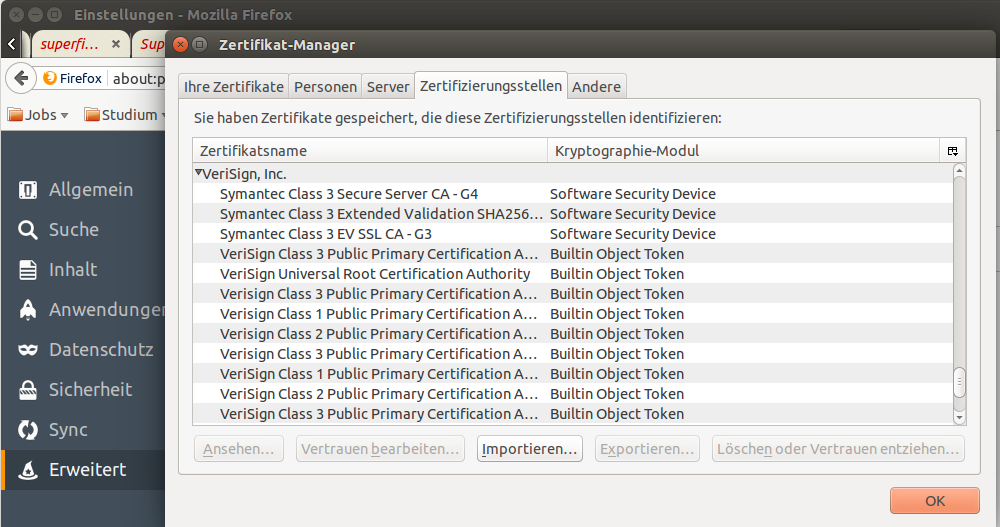
\includegraphics[width=1\linewidth]{images/firefox_installierte_zertifikate.png}
		\caption{Ausschnitt vorinstallierter Zertifikate im Firefox Browser}
\end{figure}
\noindent
Nutzt der Webservers jedoch ein selbst ausgestelltes (selbst signiertes) Zertifikat zur Authentifizierung, dann wird beim Verbindungsaufbau dem Nutzer eine Warnung angezeigt (siehe Bild ...). Der Nutzer kann anschließend selbst entscheiden ob er dem Zertifikat vertraut oder nicht. Außerdem entscheidet er ob er nur ein einziges Mal, d. h. nur für diese Verbindungssession, dem Zertifikat vertraut oder ob er eine dauerhafte Ausnahme macht. Ist letzteres der Fall, dann wird das Zertifikat im Browser installiert. Es wird dann bei den schon vorinstallierten Zertifikaten mit abgelegt. Eine dauerhafte Ausnahme hat zu Folge, dass der Benutzer beim Verbindungsaufbau zu der zugehörigen Webseite vom Webbrowser nicht mehr gewarnt wird. 
	\subsection{Sicherheitslücken bei bekannten Computer Herstellern}
Man sollte davon ausgehen können, dass die großen PC-Hersteller selbst am besten wissen müssten, wie hart der Markt in der Computerbranche umkämpft ist. Neben einer hohen Hardware-Qualität ist Kundenvertrauen immens wichtig. Zwei der weltweit bekanntesten und erfolgreichsten Computerhersteller \cite[vgl.]{pc_hersteller} haben den Faktor \textit{Vertrauen} nicht hinreichend erfüllt. Denn sowohl Lenovo als auch DELL haben das Vertrauen ihrer Kunden stark missbraucht. 

\subsubsection{Lenovo mit potentiellem Risiko}
%\subsubsection{Allgemeiner Ablauf}
Durch eine bereits vorinstallierte Software der Firma Superfish hat Lenovo versehentlich eine gravierende Sicherheitslücke auf einigen ihrer vertriebenen Notebookmodelle eingebaut. Dadurch wurde der Kunde einer zusätzlichen Gefahr eines erleichterten Hackerangriffes ausgesetzt.
%Mit der Superfish-Software beabsichtigte Lenovo, dem Nutzer gezielt personalisierte Werbung während des Surfens im Internet anzuzeigen. Um dies auch bei verschlüsselten Internetverbindungen (HTTPs) zu ermöglichen, wurde bei der Softwareinstallation auf den neuen Notebooks ein von Superfish selbst erstelltes Root-Zertifikat mit installiert. Der Kunde kaufte somit unwissentlich ein neues Notebook, auf dem ein bereits vor der Auslieferung manipuliertes Windows-Betriebssystem läuft. 
%Mit dem selbst signierten Root-Zertifikat wurden sichere (verschlüsselte) HTTPs-Verbindungen in Form einer Man-in-the-Middle Attacke aufgebrochen. Dadurch konnte sämtlicher Datenverkehr mitgelesen und  manipuliert werden. Im Fall von Lenovo geschah dies durch Einblendung von Werbung. 

%\subsubsection{Der Angriff und die benötigten Mittel}
Die Internetseite \url{www.golem.de} beschreibt die Idee und den Ablauf von den benutzerspezifischen Werbeeinblendungungen auf den Lenovo-Rechnern wie folgt: 
\begin{quote}
	\glqq Grundsätzlich ist die Idee von Superfish, dass das Programm Bilder auf Webseiten durchsucht und anhand von Algorithmen versucht zu erkennen, was sich darauf befindet. Auf Basis dessen werden dem Nutzer passende Shopping-Angebote als Werbebanner angezeigt. Geradezu zynisch wirkt die Beschreibung des Lenovo-Angestellten im Forum: Die Funktion diene dazu, Nutzern zu helfen, visuell Angebote für Produkte zu finden, bei denen sie Schwierigkeiten haben, sie mittels einer textbasierten Suchmaschine zu finden.\grqq \cite{superfish}
\end{quote}
Für die Umsetzung der Idee reichte es nicht, dass nur ein Programm von Superfish auf den Lenovo-Rechnern installiert wird. Zusätzlich benötigte Superfish unbedingt ein selbst signiertes Root-/Wurzel-Zertifikat auf dem System. Ohne dieses Zertifikat wäre es nicht möglich gewesen, auch in verschlüsselten Internetverbindungen (HTTPs-Verbindungen) den Suchalgorithmus anzuwenden, um anschließend personalisierte Werbung einzublenden. Mit dem eigenem Root-Zertifikat war Superfish in der Lage, für jede Verbindung, die zu einer HTTPs-Webseite aufgebaut wurde, ein eigenes, gefälschtes Zertifikat dynamisch zur Laufzeit zu erzeugen. Dieses wurde automatisch anerkannt, da bereits dem zugehörigen Wurzelzertifikat vertraut wurde. Weil Superfish sein Root-Zertifikat direkt im Windows-Zertifikatsspeicher installierte, wurde dieses nicht extra überprüft. Denn allen Zertifikaten, die sich im Windows-Zertifikatsspeicher befinden, wird automatisch das Vertrauen geschenkt. Der Anwender bekam dadurch nicht mit, dass keine direkte verschlüsselte Kommunikation zu dem eigentlichen Server, der die Webseite hostet, aufgebaut wurde. 
\begin{figure}[H]
	\centering
	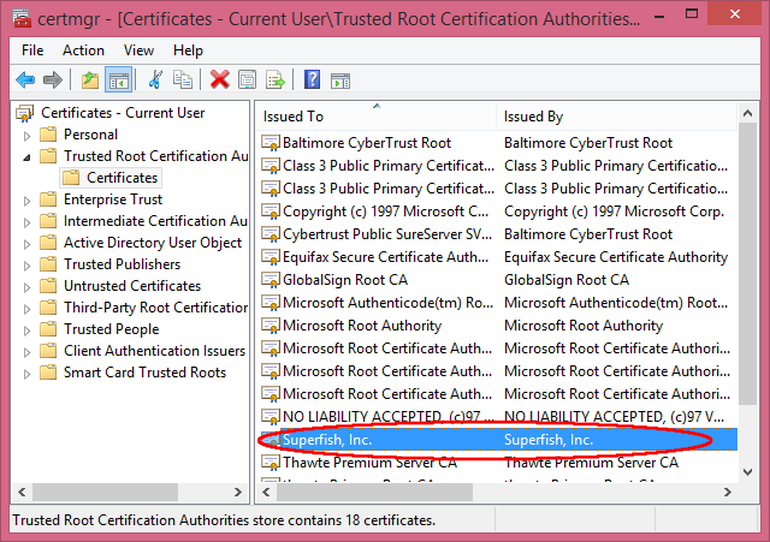
\includegraphics[width=.9\linewidth]{images/superfish.png}
	\caption{Superfish Root-Zertifikat im Windowszertifikatsspeicher, Quelle: \cite{superfish-bild}}
\end{figure}
\noindent %dadurch kein einrücken des Satzer, der nach dem Bild folgt
Weiterhin kam erschwerend hinzu, dass das Programm von Superfish für die Man-in-the-Middle Attacken ein schwaches Zertifikat nutzte. Das Root-Zertifikat verwendet für die digitale Signatur einen SHA-1 Hash-Alsgorithmus und für die asymmetrische Verschlüsselung ein 1024 Bit RSA-Verschlüsselungsverfahren. \cite[vgl.]{lenovo} Sowohl der SHA-1 Hash-Algorithmus als auch das RSA-Verschlüsselungsverfahren mit einer Schlüssellänge von 1024 Bit sind bereits erfolgreich geknackt worden und daher als unsicher einzustufen. \cite[vgl.]{sha-1,rsa}
Doch noch fataler als der Einsatz des unsicheren Hash-Algorithmus und des zu schwachen Verschlüsselungsfahrens, ist die Leichtigkeit der Entschlüsselung des privaten, geheimen Schlüssels. Robert Graham beschreibt in seinem Blog auf Errata Security eindrucksvoll, wie mit simplen Mitteln der Private Key exportiert und anschließend mit einer einfachen Wörterbuch-Attacke entschlüsselt werden konnte. \cite[vgl.]{certificate_ex}
Mittels des privaten Schlüssels kann jeder Angreifer, genau wie das Superfish-Programm, eigene, durch das Root-Zertifikat signierte, Zertifikate erzeugen und diese für bösartige Verwendungen nutzen. Somit bekommen die Anwender nicht mit, dass sie z. B. auf einer gefälschten Webseite surfen und ihre Daten ausspioniert oder manipuliert werden. Neben Zertifikaten für Webseiten, ist ein Hacker auch in der Lage, Zertifikate für kriminelle Software (z. B. Malware) zu erstellen und diese dem Nutzer als gutartig erscheinen zu lassen.  

\subsubsection{DELL mit ähnlichen Fehlern}
Der Computerhersteller DELL leistete sich einen ähnlich gravierenden Sicherheitsfehler wie sein Konkurrent Lenovo zuvor. Genau wie Lenovo hat DELL auch selbst signierte Root-Zertifikate auf einigen seiner Laptops installiert. Bei dem US-amerikanischen Hersteller sind es sogar zwei Root-Zertifikate. Sowohl das eDellRoot, als auch das DSDTestProvider Zertifikat wurden, genau wie das Superfish-Zertifikat, im Windows-Zertifikatsspeicher abgelegt. Beim Aufruf der allgemeinen Eigenschaften des eDellRoot-Zertifikats wird sogar ein Hinweis angezeigt, dass ein passender Private Key vorhanden ist. Joe Nord wendet in seinem Online-Blog die gleichen Vorgehensweisen zum Export und zur Entschlüsselung des DELL Private Keys an, wie Robert Graham beim Superfish Private Key. \cite[vgl.]{dell_joe_nord} 

\begin{figure}[H]
	\centering
	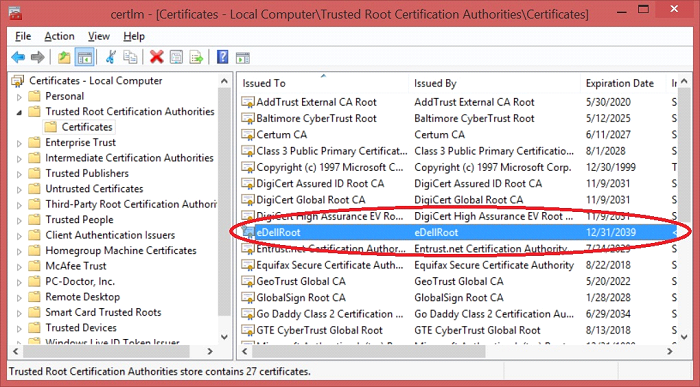
\includegraphics[width=.7\linewidth]{images/eDELLRoot.png}
	\caption{Ausschnitt aus Windowszertifikatsspeicher mit installiertem eDELLRoot Zertifikat, Quelle: \cite{dell}}
\end{figure}
	
\begin{figure}[H]
	\centering
	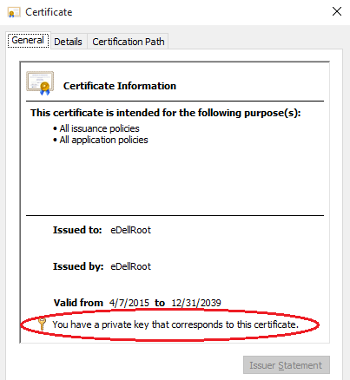
\includegraphics[width=.4\linewidth]{images/cert_eDELLRoot.png}
	\caption{Eigenschaftsansicht von eDELLRoot Zertifikat mit Hinweis auf Private Key, Quelle: \cite{dell_joe_nord}}
\end{figure}
\noindent
Angreifer mit dem privaten DELL Schlüssel haben die gleichen Angriffsmöglichkeiten auf infizierte DELL Geräte, wie Angreifer mit dem Superfish Private Key auf infizierte Lenovo Geräte.
Beide DELL Zertifikate wurden durch Software installiert, das eDellRoot Zertifikat mit dem Dell Foundation Services Programm und das DSDTestProvider Zertifikat mit der Dell System Detect Software. 
Sie sollen, laut DELL, für einfacheren Support dienen. 
DELL hat auf seiner Webseite folgende Stellungnahme publiziert: 
\begin{quote}
	\glqq[...] Das Zertifikat eDellRoot wurde zusammen mit unserer Anwendung Dell Foundation Services installiert und wird zur Unterstützung einer besseren, schnelleren und einfacheren Support-Erfahrung für unsere Kunden verwendet. Das Zertifikat ist keine Schadsoftware oder Adware. Es war ursprünglich dazu gedacht, die Service-Tag-Nummer des Systems an den Onlinesupport von Dell zu übermitteln, damit wir schnell das Computermodell identifizieren und unseren Kunden so einen unkomplizierteren und schnelleren Service bieten können. Das Zertifikat wird nicht zum Sammeln persönlicher Kundendaten verwendet. Bitte beachten Sie, dass sich das Zertifikat nicht von selbst neu installiert, nachdem es mit dem empfohlenen Dell Prozess ordnungsgemäß entfernt wurde.\\
	Wenn wir eDellRoot kennen, können wir uns auf alle unsere Anwendungen konzentrieren, die auf Dell PCs geladen werden. Wir können bestätigen, dass keine weiteren Root-Zertifikate auf dem werkseitig installierten Image installiert wurden. Wir haben jedoch herausgefunden, dass die Anwendung Dell System Detect  und das dazugehörige Root-Zertifikat DSDTestProvider ähnliche Eigenschaften hat wie eDellRoot. Im Fall von Dell System Detect lädt der Kunde die Software proaktiv herunter, um mit der Webseite vom Dell Support zu interagieren. Dadurch können wir eine bessere und individuell abgestimmte Support-Erfahrung anbieten. Wie eDellRoot auch wurde das fragliche Support-Zertifikat entwickelt, um unseren Kunden einen schnelleren und einfacheren Support zu bieten. Die Vorteile sind jedoch auf die Kunden beschränkt, die die Funktion zur Produkterkennung auf unserer Support-Webseite zwischen dem 20. Oktober und dem 24. November 2015 genutzt haben. Die Anwendung wurde von der Dell Support-Webseite sofort entfernt und es steht ab sofort eine neue Anwendung ohne das Zertifikat zur Verfügung. Wir unterstützen proaktiv ein Software-Update, um das Problem anzugehen und haben im Folgenden Anweisungen zum Entfernen des Zertifikats bereitgestellt.\grqq \cite{dell}
\end{quote}
Mit dieser Aussage hat DELL offiziell bestätigt, eigene Zertifikate auf Nutzer-Endsystemen installiert zu haben. Das eDellRoot wurde augenscheinlich bereits vor Auslieferung auf den Geräten installiert und das DSDTestProvider erst nachträglich durch Installation und Verwendung des DELL Support-Programms. Durch das DELL-Statement fällt auf, dass das eDellRoot Zertifikat sich eventuell erneut installieren kann, wenn es nicht mit spezieller DELL Software bzw. geeignetem DELL Prozess richtig deinstalliert wurde. 
\begin{quote}
	\glqq[...] Bitte beachten Sie, dass sich das Zertifikat nicht von selbst neu installiert, nachdem es mit dem empfohlenen Dell Prozess ordnungsgemäß entfernt wurde.\grqq \cite{dell}
\end{quote}
Die Ursachen für eine eventuelle Neuinstallation des DELL Zertifikats sind im nachfolgenden Kapitel \ref{sub:schutz} \nameref{sub:schutz} beschrieben.
	\section{Schutzmöglichkeiten}
Bedauerlicherweise haben Betroffene nicht allzu viele Möglichkeiten, sich gegen eben beschriebene Sicherheitslücken zu schützen. 
Eine Option wäre der Kauf von neuen Systemen ohne vorinstalliertes Betriebssystem. Wenn der Anwender selbst ein Betriebssystem nach dem Kauf installiert, kann er mit großer Sicherheit davon ausgehen, dass sich keine ungewollte, vorinstallierte Software und/oder kein selbst signiertes Zertifikat auf dem neu angeschafften Gerät befindet. Jedoch schützt diese Option nicht vor solchen Zertifikaten, die sich erst nachträglich installieren. Ein Beispiel ist das DSDTestProvider Zertifikat, welches sich beim Besuch der Support-Webseite von DELL installiert. Vorstellbar sind auch Szenarien, wo sich Zertifikate bei der Installation von Software mit einschleusen.
Eine andere Variante des Schutzes ist die regelmäßige Kontrolle der auf dem System installierten Zertifikate. Durch diese Maßnahme können auch nachträglich installierte Zertifikate entdeckt werden. Zugegeben, bei der heutigen Masse an vorhandenen, vertrauenswürdigen Zertifizierungsstellen sowie zugehörigen Zertifikaten ist es nicht leicht, den Überblick zu behalten. Erschwerend kommt hinzu, dass viele Programme zusätzlich einen eigenen Zertifikatsspeicher besitzen. Dabei kann nicht immer davon ausgegangen werden, dass diese Speicher sich auf den Zertifikatsspeicher des Betriebssystems beziehen bzw. die gleichen Zertifikate beinhalten.
Um sicherzustellen, dass mit dem richtigen Server kommuniziert wird und folglich keine Verbindung zu einer gefälschten Webseite besteht, sollte man das Zertifikat prüfen, welches für die aktuelle Kommunikation verwendet wird. Jeder Browser zeigt neben der HTTPS-Adresse ein Schlosssymbol. Über dieses Symbol werden die Eigenschaften des aktuell für diese verschlüsselte Verbindung verwendeten Zertifikats erreicht. Verschiedene Webseiten, z. B. https://globalsign.ssllabs.com, bieten eine Überprüfung der gewünschten Webseite an. Als Ergebnis zeigen sie unter anderem an, welches originale Zertifikat diese Webseite wirklich verwendet. Mittels dieser Information und der Zertifikats-Eigenschaften durch den Browser ist jeder User in der Lage zu vergleichen, ob die verschlüsselte Verbindung das richtige Zertifikat nutzt. Handelt es sich nicht um das korrekte, originale Zertifikat und gab es zusätzlich keine Fehlermeldung, so muss davon ausgegangen werden, dass keine direkte Verbindung zu der gewünschten Webseite besteht. Dies bedeutet, die verschlüsselte Verbindung wurde durch eine MITM-Attacke aufgebrochen und die Daten können mitgelesen oder sogar manipuliert werden. Nach Aufdeckung einer solchen Attacke muss das gefälschte Zertifikat im System gesucht und anschließend gelöscht werden. Dabei ist zu beachten, dass es nicht immer ausreicht nur das entdeckte Zertifikat selbst zu löschen. Da Zertifikate auf der Basis einer Public Key Infrastruktur erstellt werden, können noch weitere Zertifikate für solch eine Attacke verantwortlich sein. Es sollten, neben dem aufgespürten, gefälschten Zertifikat, zusätzlich alle anderen Zertifikate, die sich in der hierarchischen Kette befinden, überprüft und ggf. entfernt werden. Im Lenovo-Beispiel konnten mittels des gehackten, selbst signierten Root-Zertifikats weitere Zertifikate erstellt werden. Mit jedem dieser Zertifikate war anschließend eine MITM-Attacke möglich. Das Sicherheitsproblem war mit der Eliminierung des für die MITM Attacke verwendeten Zertifikats noch nicht gelöst. Erst nach erfolgreichem Entfernen des selbst signierten Root-Zertifikats konnten keine weiteren gefälschten Zertifikate erzeugt werden.
Beim DELL-Vorfall schrieb Liam Tung auf der ZDNET-Webseite: „[...] das einfache Entfernen des eDELLRoot-Zertifikats aus dem Administrator und persönlichen Zertifikatsspeicher ist nicht genug, um den Nutzer zu schützen. Einige Nutzer haben in der Tat berichtet, dass das Zertifikat nach einem Neustart wieder aufgetaucht ist.“[3]  Ursache für die Neuinstallation ist das DELL-Programm „Dell Foundation Services“, welches dieses Zertifikat verwendet. Erst mit der Deinstallation des Programms bzw. eines Plug-ins des Programms und der manuellen Löschung des DELL Zertifikats ist das selbst signierte Zertifikat dauerhaft vom System erfolgreich entfernt und die Sicherheitslücke geschlossen worden. Liam Tung schrieb zur korrekten Entfernung: „Um es dauerhaft zu entfernen und um zu verhindern, dass es sich erneut installiert, müssen Nutzer das eDELL Plugin entfernen.“ Für die detaillierte Information um welches Plugin es sich genau handelt, nutzt er die Ergebnisse von den Duo Security Forschern Darren Kemp, Michail Davidov und Kyle Lady. „‘Dies kann vollbracht werden mit Hilfe der Löschung des Dell.Foundation.Agent.Plugins.eDell.dll Moduls vom System. Geschieht dies nicht, so kann es weiterhin zur Aussetzung dieser Sicherheitslücke kommen.‘, sagte Duo Security.“ [3] Er fügte noch einen wichtigen Hinweis von Duo Security hinzu: „‘Beachte, immer wenn sie ein Werksreset auf ihrem DELL System durchführen, wird dieses Zertifikat und das eDell Plugin auf dem System wieder hergestellt und sie müssen es erneut manuell entfernen‘ [...] " [3]
Die beiden Beispiele zeigen, dass es nicht ausreicht nur die Zertifikatsspeicher auf ungewöhnliche Eintragungen zu durchsuchen, sondern ebenfalls die Programmliste des Systems auf unerwartete oder ggf. unnötig installierte Programme zu kontrollieren.
%TODO Schutz durch Client-Authentifizierung
	\subsection{Zwischenfazit}
Beide Systemhersteller nutzten ihre Position in der Marktwirtschaft und das Vertrauen, welches ihnen die Kunden entgegenbringen, schamlos aus. Sie ließen dem Käufer im Glauben, dass er ein solides Gerät mit sicherer Software gekauft hätte. Doch ohne selbständige Gegenmaßnahmen des Kunden war dieser, mittels der von Lenovo und DELL selbst signierten Zertifikate, potentiellen Angreifern hilflos ausgesetzt. Die Käufer müssen auf der einen Seite für die Zukunft hoffen, dass die Gerätehersteller aus ihren Fehlern gelernt haben und wieder sichere Systeme herstellen bzw. verkaufen. Auf der anderen Seite kann und sollte jeder selbständig Kontrollen und Überprüfungen durchführen. Außerdem ist es ratsam, sich ein wenig mit den Systemen zu befassen mit denen man täglichen Umgang hat und wichtige Tätigkeiten, wie z. B. Online Banking, durchführt. Darunter zählt auch das regelmäßige Abrufen von Informationen über Sicherheitsneuigkeiten in bekannten Sicherheitsforen, z. B. \url{https://www.heise.de/security}
\\
\\
Gemäß dem Sprichwort „Vertrauen ist gut, Kontrolle ist besser.“, sollte jeder Benutzer, mit den verfügbaren Möglichkeiten, die verwendeten Systeme und Dienste immer wieder überprüfen.

	\newpage
	
	%% Diana
	\subsection{Was ist ein geswitchtes Netz?}
\label{sec:geswitchtes_netz}
Ein geswitchtes Netzwerk zeichnet aus, dass die Auslastung des Netzwerke durch den Datenfluss der Netzwerkteilnehmer stark reduziert wird, da ein Frame nur an die Ziel-Adresse gesendet wird, wenn sie bereits in der Switch-Tabelle hinterlegt ist.

Somit bringt der Einsatz eines Switches auch mehr Sicherheit, wenn es darum geht, wer im Netzwerk hängt und wer welche Daten erhalten soll.

Ein Switch kann Netzwerkteilnehmer auch in Gruppen aufspalten und hier unterscheiden, an welche Gruppe das Frame zugestellt werden soll, das Verhalten ist wie bei zwei getrennten LAN.
Die Netzwerkteilnehmer sehen dann nur die Frames in ihrer Gruppe.

\begin{figure}[H]
	\centering
	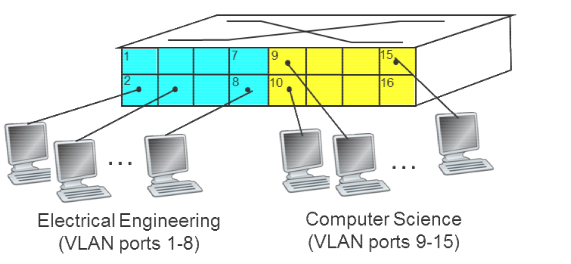
\includegraphics[width=0.7\linewidth]{images/VLAN_1.png}
	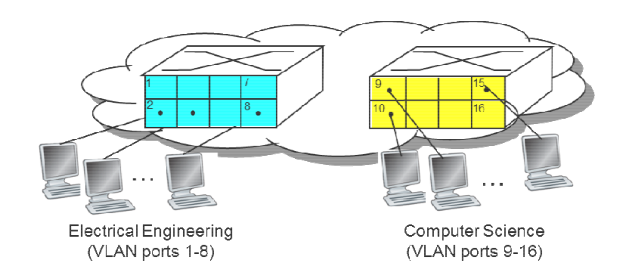
\includegraphics[width=0.8\linewidth]{images/VLAN_2.png}
	\caption{Zusammenfassung der Ports eines Switches zu einzelnen Gruppen \cite[Kapitel 5, Abbildung Folie 41]{netzwerkeI}}
\end{figure}

Jedes Netzwerk verfügt heutzutage über mindestens einen Switch, da mehrere Netzwerkteilnehmer zu besser verwaltet werden können.
Früher hat diese Aufgabe ein Hub oder eine Bridge übernommen, bis diese vom Switch abgelöst wurden.
\begin{figure}[H]
	\centering
	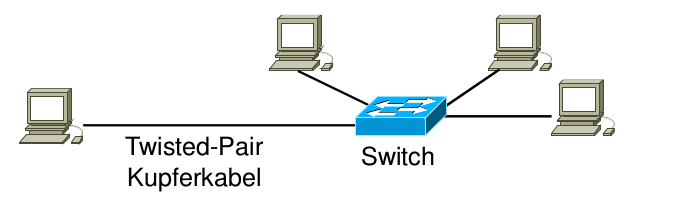
\includegraphics[width=1\linewidth]{images/geswitchtes_netz.png}
	\caption{Geswitchtes Netzwerk \cite[Kapitel 5, Abbildung Folie 33]{netzwerkeI}}
\end{figure}
\subsubsection{Mehrere Switches in einem Netzwerk}
Mehrere Switches in einem Netzwerk sind natürlich möglich, allerdings kann man diese nicht einfach so miteinander verbinden, sonst entsteht eine Schleife.
Ist eine Schleife in einem Netzwerk gelegt, bricht der gesamte Datenverkehr zusammen.

Für die Umsetzung mehrerer Switches in einem Netz müssen ein paar Vorkehrungen getroffen werden, unter anderem spezielle Kabel.




	


	%% Was so alles in einen Anhang kommt
	%\appendix
	
	\newpage
	\phantomsection
	\addcontentsline{toc}{section}{Literatur}
	\bibliography{literatur}
	
	
	
\end{document}